The objective addressed in this Section is to develop a procedure to
identify spectral bands that yield good temperature, gravity and
metallicity diagnostics. Given the lack of a calibration set of
observed spectra with homogeneous coverage of the space of physical
parameters, we turn to synthetic libraries of spectra. Furthermore,
only temperatures and gravities can be calibrated independently of the
spectra: all metallicity estimates in the literature are based on
collections of synthetic spectra, and therefore spectral synthesis
codes are the only resource to construct regression models.

The atomic or molecular line/band parameters could in principle
indicate the spectral features that are more sensitive to changes in
the physical parameters. The suitability of spectral features as
diagnostics ofthe stellar atmospheric properties depends not only on
the individual behaviour of each line/band, but also on the relative
properties of neighbouring features in the same spectral region, that
may overlap depending on the spectral resolution. Furthermore, good
spectral diagnostics at a given signal-to-noise ratio (SNR) may show a
severely degraded predictive power in the low SNR regime. In the
following we adopt the BT-Settl library of synthetic spectra
(\cite{2013MSAIS..24..128A}) as the framework where spectral
diagnostics will be searched for. These synthetic spectra were
pre-processed in several steps as described below.

\subsection{Spectral preprocessing}

First, and in order to define good temperature diagnostics, spectra
between 2000 and 4200K in steps of 100 K were selected, with $\log(g)$
in the range between 4 and 6 dex (when g is expressed in cm/s$^{-2}$),
in steps of 0.5 dex. The metallicity of the representative spectra was
restricted to the set 0, 0.5 and -1 dex.  This yields a total set size
of 535 available spectra.

A series of preprocessing steps were then carried out in order to
match the spectral resolution and wavelength coverage and sampling of
the synthetic library to that of the collection of observed spectra
(IPAC or IRTF, see below). This required the definition of a common
wavelength range present in all available observed spectra, and the
subsequent trimming to match that range. A unique wavelength sampling
was also defined and all spectra (synthetic and observed) interpolated
to match the sampling. Finally, all spectra, both synthetic and
observed were divided by the integrated flux in order to factor out
the stellar distance.

%%%%%%%%%%%%%%%%%%%%%%%%%%%%%%%%%%%%%%%%%%%%%%%%%%%%%%%%%%%%%%%%%%%%%%%%%
%                          TO BE REMOVED
%%%%%%%%%%%%%%%%%%%%%%%%%%%%%%%%%%%%%%%%%%%%%%%%%%%%%%%%%%%%%%%%%%%%%%%%%
%In order to increase the density of examples in parameter space, we
%introduced interpolated spectra in the BT-Settl grid. Interpolation
%was obtained as a linear combination of spectra in the grid, weighted
%by the inverse square of the euclidean distance. {\bf Aqui, la
%distancia euclidea deberia calcularse en parametros normalizados,
%porque si no la temperatura domina la distancia. Fue asi?} We compared
%a set of interpolated spectra with those produced using the PHOENIX
%code (\cite{fuhrmeister2005phoenix}) to be sure that interpolation was
%a valid solution to infer new synthetic spectra. {\bf Yo aqui daría el
%RMSE de reconstruccion, mejor que la figura comp-gen-inter}

%(see Fig.~\ref{fig:comp_gen_inter}).  }

%\begin {figure}
% \begin{center}
% 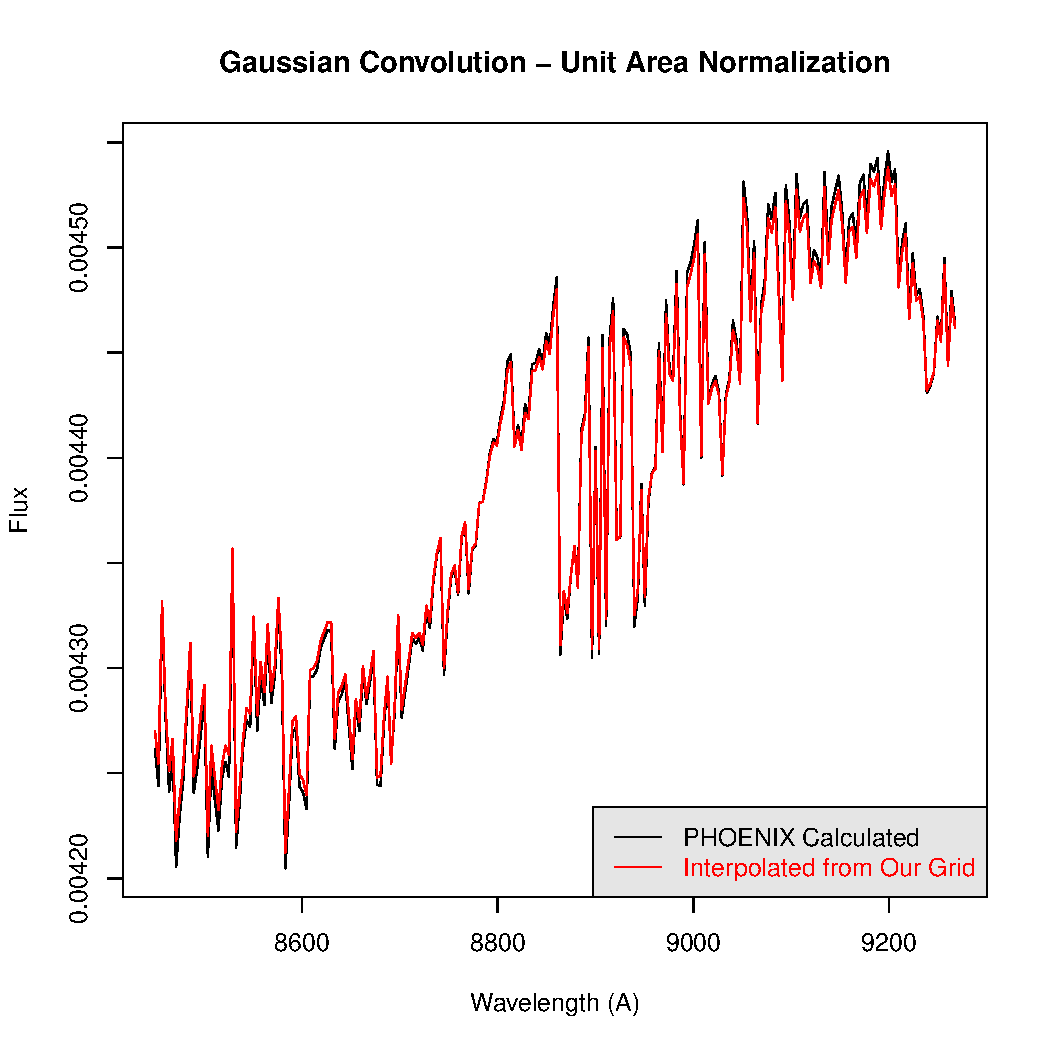
\includegraphics[width=6cm]{figs/intgrid4_gauss.pdf}
% \caption{Comparison between generated and interpollated spectrum}
% \label{fig:comp_gen_inter}
% \end{center}
%\end {figure}

%A first interpolation stage allowed us to define a finer mesh step of
%0.25 dex for both, $\log(g)$ and metallicity and 50K in temperature,
%yielding a total 1329 spectra.  Then, a second interpolation stage
%refined the grid down to 25 K in temperature and 0.125 dex in
%$\log(g)$, keeping the metallicity step at 0.25 dex and producing a
%dataset with 25912 spectra.  In spite of these, and in order to keep
%their knowledge closer to the original BT-Settl source, most of the
%analyses have been performed with the original 535 spectra
%dataset.{\bf Habría que delimitar exactamente donde se han utilizado
%535 y dónde 25912. Si la mayoria del analisis se ha realizado sobre
%535, no se si tiene sentido incluir la parte de interpolacion.}
%%%%%%%%%%%%%%%%%%%%%%%%%%%%%%%%%%%%%%%%%%%%%%%%%%%%%%%%%%%%%%%%%%%%%%%%%%

In order to avoid selecting spectral features that are good predictors
only in the unrealistic SNR=$\infty$ regime, the search for optimal
diagnostics of the atmopheric paramters of M stars was carried out for
three SNR values (10, 50 and $\infty$) by degrading the synthetic
spectra with Gaussian noise of zero mean. These values were found to
be sufficient in a wide range of experiments carried out in parallel
and described in \cite{Anaetal}.

\subsection{Feature definition and selection}
\label{subsec:FD}
As mentioned in Sect. \ref{sec:intro}, it is well known the
difficulty in defining good spectral diagnostics for M stars in the
infrared.

The work in \cite{cesetti} defined wavelength regions in the I and K
bands optimal for the diagnostic of physical parameters based on the
sensitivity exhibited by the flux emitted in these segments to changes
of the physical parameters. The sensitivity was measured in terms of
the derivative of the flux with respect to the physical parameter. The
approach adopted in this work is to select spectral features that
yield the best accuracy when used as predictive variables in a
regression model that estimates the stellar atmospheric physical
parameters ($T_{eff}$, $\log(g)$ and metallicity). The evaluation of
the accuracy of the estimates produced from a subset of features is
described further below. We consider the effective temperature as the
dominant parameter influencing changes in the stellar spectra (a
strong feature) and thus, it was estimated first, and then used as in
the regression models for the gravity and metalicity.

Here, a feature $F$ is defined as

\begin{equation}\label{eq:featureDefinition}
  F = \int_{\lambda_{1}}^{\lambda_{2}} (1-\frac{f(\lambda)}{F_{cont}} \cdot {\rm d}{\lambda})
\end{equation}

where $f(\lambda)$ denotes the normalized flux from the star at
wavelength $\lambda$, and where $F_{cont}$ is the average flux in a
spectral band between $\lambda_{cont;1}$ and $\lambda_{cont;2}$. We
explain below how we search for the band definitions that produce
physical parameter predictions with the smallest errors.

Another type of features defined as

\begin{equation}\label{eq:feature2}
  F' = \frac{ \int_{\lambda_{1}}^{\lambda_{2}}f(\lambda) \cdot {\rm d}{\lambda}}
               {\int_{\lambda_{3}}^{\lambda_{4}} f(\lambda) \cdot {\rm d}{\lambda}} 
\end{equation}

was considered, where $\lambda_1, \lambda_2, \lambda_3$, and
$lambda_4$ delimit two spectral bands such that the ratio of the
integrated fluxes in the two bands is hoped to be a good predictor
(alone or in combination with other features) of the star atmospheric
physical parameters. The results obtained with this alternative
feature definition did not differ significantly on average from the
ones observed with the one adopted in Eq. \ref{eq:featureDefinition}, and
including them here would result in an excessively lengthy paper. In
view of the equivalent global performances, we prefered the former
because it allows direct comparison with the features proposed
by \cite{cesetti}.

We used Genetic Algorithms to solve the optimization problem described
above, that is, the problem of finding the features (band boundaries)
that minimize the prediction error of a regression estimate of the
physical parameters. We used the implementation of genetic algorithms
publicly available as the R \citep{R2013} ???  package. The concept of
using in-silico evolution for the solution of optimization problems
was introduced by \cite{holland1975adaptation}. Although its
application is now reasonably widespread \citep[see
e.g. ]{goldberg1989genetic}), they became very popular only when
sufficiently powerful computers became available. {\bf Aquí hay que
citar trabajos en astrofísica que utilicen GA y, en particular, un
artículo de Charbonneau
http://adsabs.harvard.edu/abs/1995ApJS..101..309C en 1995 que fue como
la presentación en sociedad.}

For the sake of simplicity let us define Genetic Algorithms (GAs) as
search algorithms that are based on the principle of evolution by
natural selection. The procedure works by evolving (in the sense
explained below) sets of variables (chromosomes) from an initial
random population. Evolution proceeds via cycles of differential
replication, recombination and mutation of the fittest
chromosomes. The concept of fittest is context dependent, but in our
case fitness is defined in relation with the accuracy with which a
given chromosome (set of spectral features ${F_i}$) predicts the
physical parameters.

The implementation of the GA comprises the following steps:

\begin{itemize}
\item [\textbf{Stage 1}:]{Definition of the population of potential features (chromosomes).}
\item [\textbf{Stage 2}:]{Each chromosome in the population is evaluated by its ability to
predict the physical paramters of each star in the dataset (fitness
function).}
\item [\textbf{Stage 3}:]{Chromosome selection, when a chromosome has 
 a score higher than a predefined value.}
\item [\textbf{Stage 4}:]{The population of chromosomes is replicated. 
 Chromosomes with higher fitness scores will generate more numerous
 offspring.}
\item [\textbf{Stage 5}:]{The genetic information contained in the replicated parent
chromosomes is combined through genetic crossover. Two randomly
selected parent chromosomes are used to create two new chromosomes.}
\item [\textbf{Stage 6}:]{Mutations are then introduced in the chromosome randomly. 
 These mutations produce new genes used in chromosomes.  Steps 5 and 6
 are applied over the chromosomes established at Step 4.}
\item [\textbf{Stage 7}:]{This process is repeated from Stage 2 until 
  a target accuracy is achieved or the maximum number of iterations is
  attained.}
\end{itemize}

We test features (both for the numerator and denominator of
Eq. \ref{eq:featureDefinition}) that comprise ten consecutive spectral
bins of the spectrum. These features may overlap by as much as 5
consecutive bins (which in practice implies that we define the first
feature as the spectral chunk between wavelength bins $i=1$ and
$i=10$, the second feature between bins $i=6$ and $i=15$, the third
feature between bins $i=11$ and $i=20$, etc). We do not test for
feature ratios that overlap in wavelength.

{\bf The distribution of the ratio of two gaussian variables (our
case) has extremely wide wings if any of the features is centred
around zero. We should automatically discard features like this. Can
we do it now?}

An obvious conceptual limitation of a univariate approach (considering
chromosomes that code a single predictive feature) would be the lack
of consideration that features work in the context of interconnected
pathways and, therefore, it is their behavior as a group that has to
be evaluated in terms of the predictive accuracy. Multivariate
selection methods thus seem more suitable for the analysis of the
regressors since variables are tested in combination to identify
interactions between features. In this work we define a chromosome as
a set of ten individual genes, and each gene codes a pair of
non-overlapping spectral bands, the ratio of which is used as
predictor of the physical parameters according
to \ref{eq:featureDefinition}. 

The population size was set to 8000 individuals and the maximum number
of accepted iterations set to 4000. We produced three randomly started
populations so as to provide enough initial variety. The crossover and
mutation probabilities were set to 0.85 and 0.35 respectively. Elitism
was fixed to 0.15 {\bf No hemos mencionado elitismo; hay que
mencionarlo y definirlo antes}.

Feature fitness was defined in terms of the Akaike Information
Criterion (AIC) for linearity between the potential feature against
the physical parameter.

The most frequent and efficient features were selected as candidates
to predictive variables of the physical parameters in regression
models. We used a binary codification of the chromosomes and a
parallel implementation of the GA in a farm of fifteen computers per
physical parameter. {\bf Here a bit more detail is needed: what
processors, number of cores, etc. Just one additional sentence.}

The GA procedure provides us with a large collection of chromosomes.
Although these are all potential solutions of the problem, it is not
immediately clear which one should be selected for the final
regression model.  This single regression model should, to some
extent, be representative of the population. The simpler strategy
would be to use the frequency of the chromosome in the population as
criterion for inclusion in a forward selection strategy. However we
prefered to select the features based on their highest fitness. {\bf
How many? Do we select the top 10 fittest chromosomes? Why 10?}

Once the GA has generated a proposal set of features for predicting
each of the physical parameters, the next step consists in training
the regression model to predict them based in these features.  The GA
generates a large set of proposals {\bf here we need to explain how we
go from the output of the GA to a list of 10 features. They are
ordered by fitness and number of replicates in the pool, I believe. We
keep the top fittest features with many replications, but can we
describe this more quantitatively?}

There are different statistics that can be used to identify features
that are differentially expressed between two or more groups of
samples {\bf hay que explicar a qué nos referimos con differential
expression, samples y groups of samples aquí} and then uses the most
differentially expressed ones to construct a statistical model.

In order to assess the performance of the regression models, we
compare their predictions with i) values of the physical parameters
from the literature (when available); ii) the predictions from the
popular $minimum \chi^2$ distance to spectra in the BT-Settl library;
iii) parameter predictions based on a projection pursuit regression
model {\bf Is this correct, Joaquín? Somewhere in your first version
of the paper it was stated that the ICA components were fed to an SVM
with C=10 and epsilon=0.001 for temperature, and different values for
logg and metallicity} trained with projections of the BT-Settl spectra
onto the set of vectors resulting from an Independent Component
Analysis (ICA); and finally, iv) predictions from a regression model
trained with the features proposed by \cite{cesetti} (only for the
IRTF spectra) {\bf Joaquín, aquí necesitamos explicar qué tipo de
modelo entrenamos con las features de cesetti.}.

\subsection{Models considered.}
\label {ssub:models}
For the models to be built, the same strategy was used for all the
three physical parameters $(T_{eff}, log(g), met)$ and it was to use
non linear methods for modellization.  As a classical regression
problem several linear and non-linear modelling techniques with
specific research for adequate parameters per method when required,
were considered: {\bf Joaquín, no entiendo este párrafo. Pareces decir
primero que utilizas modelos no lineales, para luego indicar que
utilizas varios modelos lineales y no lineales. Los GAMs son lineales
¿no?}

\begin{itemize}
 \item {Generalized Additive Models \emph{(GAM)}.}
 \item {Bagging with Multiadaptative Spline Regression Models \emph{(MARS)}.}
 \item {Random Forest Regression Models \emph{(RF)}.} 
 \item {Gradient Boosting with Regression Trees \emph{(BOOSTING)}.}
 \item {Generalized Boosted Regression Models \emph{(GBM)}.}
 \item {Support Vector Regression with Gaussian Kernel \emph{(SVM)}.}
 \item {MLP Neural Networks \emph{(NNET)}.}
 \item {Kernel Partial Least Squares Regression \emph{(KPLS)}.}
 \end{itemize}


Including here a sufficient description of each and every regression
model that we trained would render the manuscript excessively
lengthy. Suffice it to say that each one of them can be thought of as
a parametric model that predicts one physical parameter from an input
vector. The input vector can be the full normalised spectrum, the ICA
lower-dimensional representation of the full spectrum, or the spectral
features selected by \cite{cesetti} or by the GA. The model parameters
are infered (using algorithms that differ from one regression model to
the other) from a set of examples. This set of examples (spectra of
stars for which we know the physical parameters) is called the
training set, and the process by which the model parameters are
determined from the training set, is called training of the model. In
the next paragraph we give minimal details of each regression model
trained, and references for the interested reader.

{\bf Aquí haría falta describir muy mínimamente cada uno de los
modelos y dar una referencia que los describa en detalle. Luego,
explicar cómo se determina el valor óptimo de los parámetros de cada
modelo. Me pareció entender que caret lo hace automáticamente, pero en
cualquier caso habría que escribirlo explícitamente y citar caret (si
este es el caso).}

As mentioned above, the training set was constructed from the BT Settl
library of stellar spectra. The interested reader may find different
approaches in the literature to the problem of finding an optimal set
of training examples. \cite{hoggCannon} for example prefer to use real
observed spectra rather than synthetic libraries to create a
generative model in which the individual spectral fluxes are modelled
as second degree polynomials with the physical parameters as
arguments. The real observed spectra have physical parameters taken
from the literature, which in turn are almost always inferred using
synthetic spectral libraries. In our opinion, this approach does not
solve the dependence of the predicted parameters on the necessarily
imperfect synthetic libraries, but has the advantage that the relative
frequencies of examples in the training set represents better the
biases naturally encountered in surveys than the uniform sampling of
parameter space found in synthetic libraries. Recently, \cite{heiter}
have started a program to compile a set of stars with accurate
physical parameter determinations infered independently of
spectroscopic measurements and atmospheric models (as much as
possible). Unfortunately, this ambitious program only contains 34
stars of spectral types F, G, and K. In the M regime we find similar
approaches in \cite{dummy}, \cite{dummy}, and \cite{dummy}, where the
atmospheric parameters are derived using interferometric measurements
of stellar radii. Again, this only amounts to a very small number of
examples and a very sparse sampling of the parameters space.

We believe that all efforts to compile training sets of stars with
accurate, homogeneous, and reliable physical parameters derived
independently of spectroscopic measurements are valuable not only
because they allow for the improvement of the stellar atmospheric
models but also because they help increase the reliability of the
regression models by making them independent of these same atmospheric
models. But until these training sets with sufficient and homogeneous
sampling of the parameter space are available, we turn to the use of
synthetic libraries. 

